
\documentclass[chaptersright]{informeutn}
\usepackage[utf8]{inputenc}
\usepackage{array}
\usepackage{geometry}
\usepackage[table]{xcolor}
\usepackage{colortbl}
\usepackage{caption}
\usepackage{graphicx}

\materia{Dispositivos Electronicos I}
\titulo{Trabajo Practico N°3: BJT}
\comision{3R2}
\autores{Documentador y operador: Angelo Prieto 401012\\ Coordinador: Gaston Grasso 401892}
\fecha{24-06-2025}

\begin{document}
\maketitle
\tableofcontents

\chapter{Introduccion}

\chapter{Identificación de las zonas de trabajo del transistor}
  \section{Zona de corte}
    \subsection{Actividad de simulación}

  \section{Polarizacion de la juntura Base-Emisor}
    \subsection{Actividad de laboratorio}
      \begin{center}
      \resizebox{\textwidth}{!}{%
        \begin{tabular}{|c|c|c|c|c|c|c|c|c|c|c|c|}
          \hline
          $V_{BB}$ & 0 & 0.3 V & 0.4 V & 0.5 V & 0.6 V & 0.7 V & 0.8 V & 1 V & 3 V & 7 V & 10 V \\
          \hline
          $I_B$ & 0 A & 29 nA & 43 nA & 91 nA & 0.78 uA & 4.99 uA & 12.46 uA & 35.84 uA & 226.3 uA & 625 uA & 929 uA \\
          \hline
          $V_{BE}$ & 0 V & 0.27 V & 0.38 V & 0.48 V & 0.57 V & 0.63 V & 0.66 V & 0.68 V & 0.73 V & 0.75 V & 0.75 V \\
          \hline
        \end{tabular}%
      }
      \end{center}
      
      \begin{figure}[h]
        \centering
        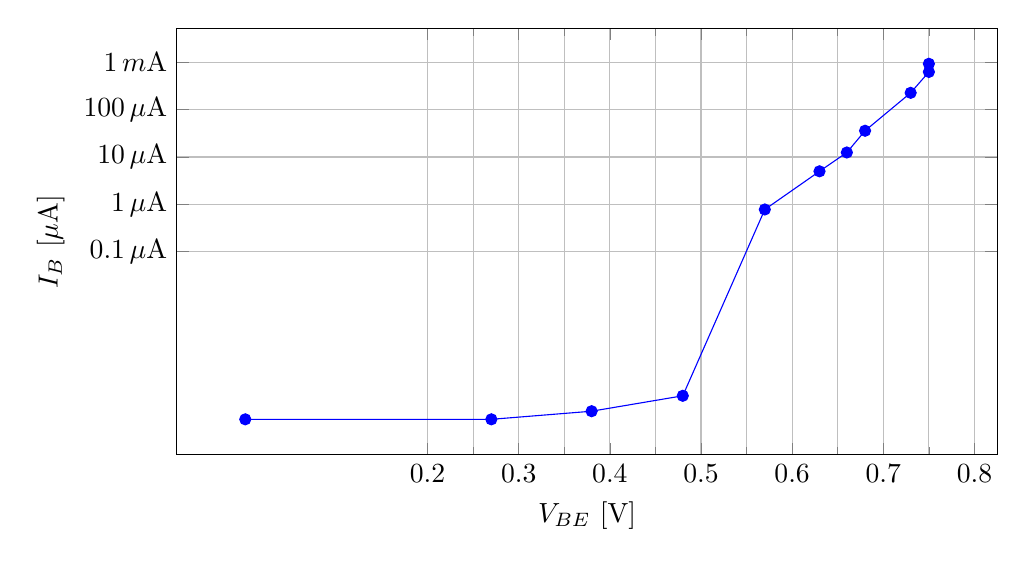
\begin{tikzpicture}
        \begin{axis}[
          width=12cm,
          height=7cm,
          xlabel={$V_{BE}$ [V]},
          ylabel={$I_B$ [$\mu$A]},
          grid=both,
          minor tick num=1,
          xtick={0.2,0.3,...,0.8},
          ymode=log,
          log basis y=10,
          ytick={1e-4,1e-3,1e-2,1e-1,1,10,100,1000},
          yticklabels={$0.1\,\mu$A,$1\,\mu$A,$10\,\mu$A,$100\,\mu$A,$1\,m$A}
        ]
        \addplot[
          mark=*,
          color=blue
        ] coordinates {
          (0.00, 0.000000029)
          (0.27, 0.000000029)
          (0.38, 0.000000043)
          (0.48, 0.000000091)
          (0.57, 0.00078)
          (0.63, 0.00499)
          (0.66, 0.01246)
          (0.68, 0.03584)
          (0.73, 0.2263)
          (0.75, 0.625)
          (0.75, 0.929)
        };
        \end{axis}
        \end{tikzpicture}
        \caption{$I_B$ en función de $V_{BE}$}
      \end{figure}


\chapter{Curvas características}

\chapter{Caracteristicas de transferencia de corriente}

\chapter{interpretacion de las especificaciones del fabricante}

\chapter{conclusiones}


\end{document}
